\level{2}{AHalGenRampUpDown}

\level{3}{Structure}
{
\centering{}
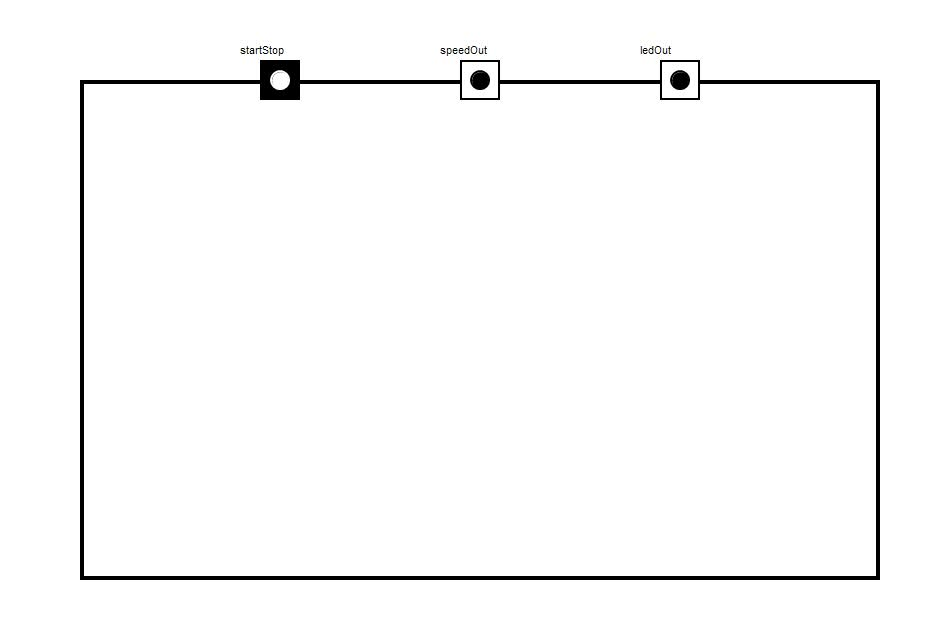
\includegraphics[width=1.0\textwidth]{./images/AHalGenRampUpDown_structure.jpg}
\figcaption{AHalGenRampUpDown Structure}
}

\level{3}{Ports}
\begin{tabular}[ht]{|l|l|l|l|l|p{5cm}|}
\hline
\textbf{Name} & \textbf{Protocol} & \textbf{Type} & \textbf{Kind} & \textbf{Multiplicity} & \textbf{Description}\\
\hline
startStop & POnOff & reg. & external & 1 & \\
\hline
speedOut & PSpeed & conj. & external & 1 & \\
\hline
ledOut & POnOff & conj. & external & 1 & \\
\hline
\end{tabular}

\level{3}{Behavior}
\level{4}{Top Level}
{
\centering{}
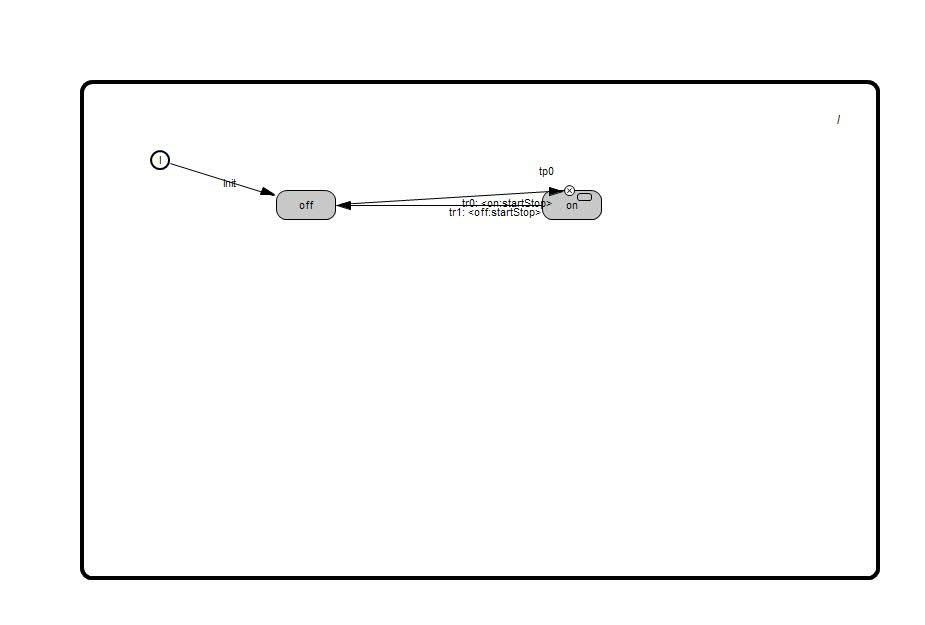
\includegraphics[width=1.0\textwidth]{./images/AHalGenRampUpDown_behavior.jpg}
\figcaption{AHalGenRampUpDown Top State}
}

\begin{par}

\end{par}

\level{4}{Subgraph on}
{
\centering{}
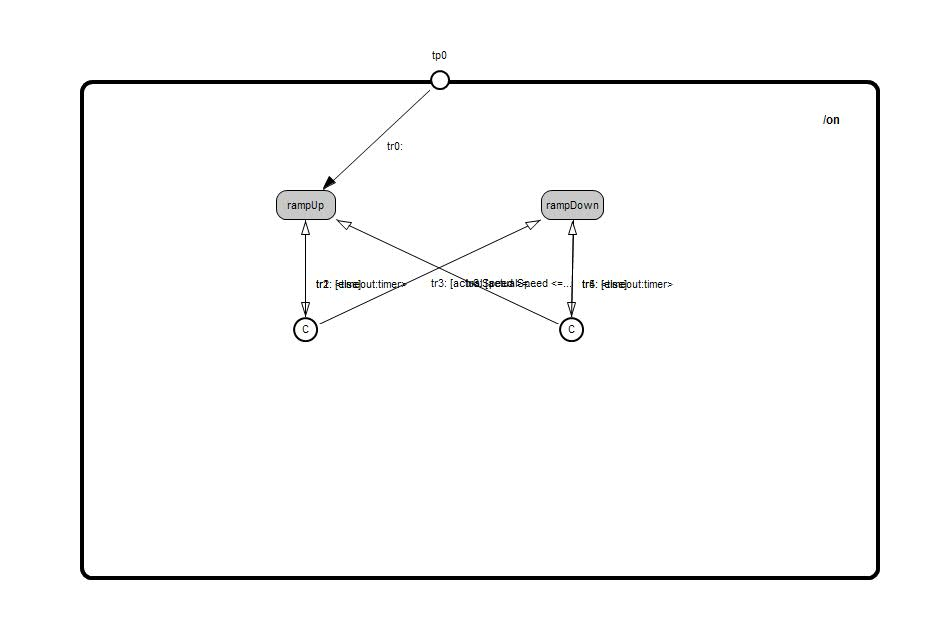
\includegraphics[width=1.0\textwidth]{./images/AHalGenRampUpDown_on_behavior.jpg}
\figcaption{AHalGenRampUpDown\_on}
}

\begin{par}

\end{par}
	

\level{3}{Attributes}
\begin{tabular}[ht]{|l|l|p{8cm}|}
\hline
\textbf{Name} & \textbf{Type} & \textbf{Description}\\
\hline
speedStep & uint32 & \\
\hline
timeStep & uint32 & \\
\hline
minSpeed & uint32 & \\
\hline
maxSpeed & uint32 & \\
\hline
actualSpeed & uint32 & \\
\hline
\end{tabular}

